\chapter{这是第一章}

\section{第一章第一节}
这是第一章第一节

\subsection{第一章第一节第一小节}
毕业论文只允许使用三级标题,再要写字标题可以成编号的形式:
一个回车不换行

两个回车才换行。
\begin{enumerate}
\item 编号一
\item 编号二
\item 编号三
\end{enumerate}
还可以自定义编号的形式:
\begin{enumerate}[自定义1:]
\item 编号一
\item 编号二
\item 编号三
\end{enumerate}
\section{公式}
公式编写使用标准的{\LaTeX}公式语法,可以参考这个网址\url{https://www.latexlive.com/}。引用格式为:式(\ref{eq1-1}),式(\ref{eq1-4})。行内公式可用$A_2$
\begin{equation}
\left \{ \begin{aligned}
\dot U_1 &=  - {{{U_1}} \over {{R_1}{C_1}}} + {{{I_L}} \over {{C_1}}} \\
U_L &= {U_{oc}} - {U_1} - {I_L}{R_0}
\end{aligned}
\right.
\label{eq1-1}
\end{equation}

\begin{equation}
SOC= {Q_{pre} \over Q_{max}}\times 100\% \label{eq1-4}
\end{equation}

\section{图片}
插入图片显示如下,引用\figref{fig5-1},scale可以直接调整比例。[H]代表浮动体,删除则图片和表格自动调整,默认总是在页面最上方。
\begin{figure}[H]
\centering
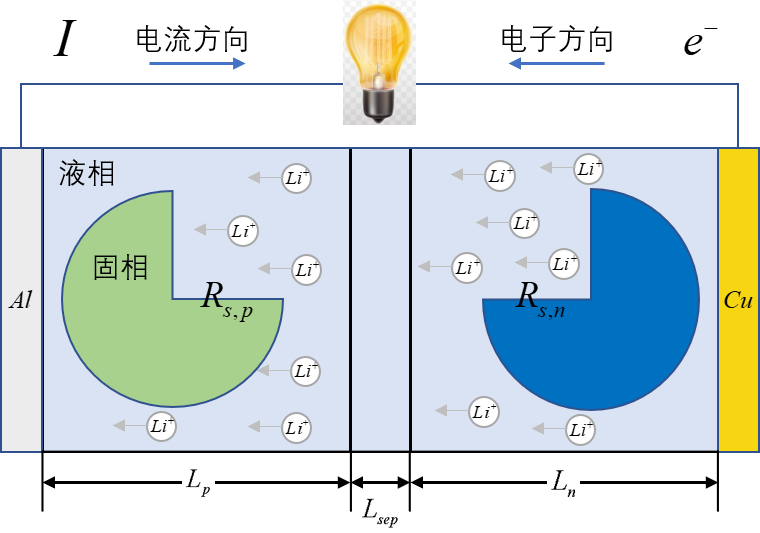
\includegraphics[scale=0.75]{figure/chap1/Li-ion.png}
\caption{FOMe原理示意图}
\label{fig5-1}
\end{figure}
也可设定长宽数值调整图片大小,如\figref{fig1-2}所示。
\begin{figure}[H]
\centering
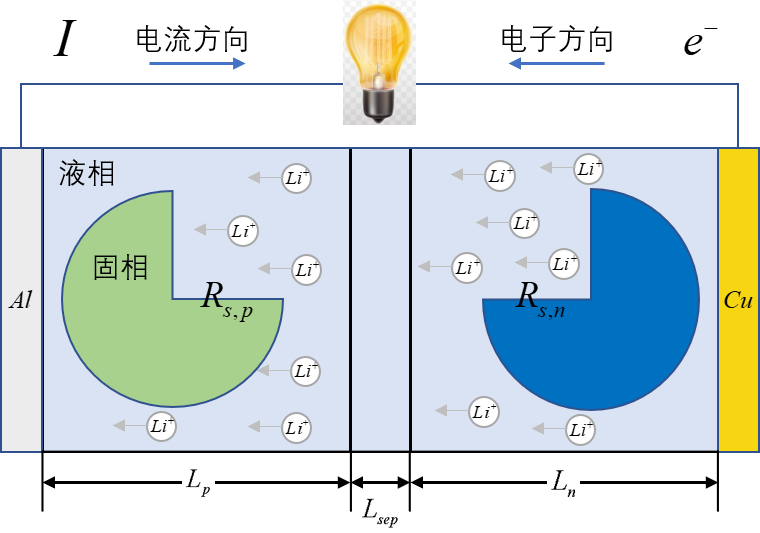
\includegraphics[width=6cm,height=6cm]{figure/chap1/Li-ion.png}
\caption{width=6cm,height=6cm}
\label{fig1-2}
\end{figure}

\section{表格}
表格使用方法如下,引用格式:如\tabref{tab1-1}
\begin{table}[H]%[htbp]
	\centering
	\begin{spacing}{1.35}
		\caption{锂离子电池、镍氢电池和铅酸电池性能对比}
		\label{tab1-1}
		\begin{tabular}{|m{2.5cm}<{\centering}|m{3.2cm}<{\centering}|m{3.2cm}<{\centering}|m{3.2cm}<{\centering}|}
			\hline
			特性  & 锂离子电池 & 镍氢电池 & 铅酸电池  \\%\tabincell{c}{阶乘数\\(十进制形式)} \\
			\hline
        工作电压(V) & 3.6 & 1.26 & 2 \\ \hline
        循环寿命(周次) & ≥800 & ≥500 & ≥300 \\ \hline
        自放电率(\%/月) & 5 & 20 & 30 \\ \hline
        环保性 & 不含重金属,相对传统电池更环保 & 含有重金属,不如镍氢电池和锂离子电池环保 & 不含重金属,相对于铅酸电池更环保 \\ \hline
		\end{tabular}
	\end{spacing}
\end{table}

三线表如\tabref{tab2-8}
\begin{table}[h!]
\centering
\begin{spacing}{1.35}
\caption{FOM,FOMe与P2D模型仿真耗时}
\label{tab2-8}
\begin{tabular}{cm{2.5cm}<{\centering}}
\toprule[1pt]
	电化学模型 	&	计算时间        \\
\midrule[0.5pt]
FOM &         0.3742s    \\
FOMe	&       0.3964s    \\
P2D   &   42s  \\
\bottomrule[1pt]
\end{tabular}
\end{spacing}
\end{table}

这个网址\url{https://tableconvert.com/zh-cn/excel-to-latex}提供了Excel表转{\LaTeX}格式的表。
